% FILLED (fill batch): process ⑥ Confinement — Ioffe-Pritchard magnetic
%   minimum trap (RTSC/Wheeler inherited).
%   folds stdlib ioffe_loop_bz / _mirror_bmin / _bcoil / _deltab /
%   _trap_depth_k / mu_b_over_kb (PR #168) + the inherited Wheeler on-axis
%   current-loop closed form + the mirror-pair superposition + negative
%   control, from companion/verify-ledger.json.
\section{Confinement --- the Ioffe--Pritchard Magnetic-Minimum Trap}
\label{app:confinement}

This appendix is the full data record for pipeline process
\textcircled{\scriptsize 6}, where the funnel inherits its magnetostatic
kernel from the sibling RTSC magnet domain (Appendix~\ref{app:rtsc}). We
state the inherited on-axis current-loop closed form, the two-coil mirror
superposition that produces a genuine on-axis $|B|$ minimum, the trap depth
and its load-bearing constant $\mu_B/k_B$, and the reference mirror pair.
Every digit traces to PR~\#168 and the seven \texttt{ioffe\_*} /
\texttt{mu\_b\_over\_kb} atoms (plus one \tierRed\ control) in
\texttt{companion/verify-ledger.json}.

% -------------------------------------------------------------------------
\subsection{Why a magnetic minimum}
\label{app:conf-why}

Ground-state antihydrogen is electrically neutral, so it cannot be held by
the electrostatic fields of a Penning trap. What remains is the magnetic
moment $\mu\approx\mu_B$ of the bound positron: a low-field-seeking state has
potential energy $U=+\mu|B|$, so it is pushed toward \emph{weak} field. A
trap must therefore be a region where $|B|$ has a local \emph{minimum} at the
centre and rises in every direction --- a magnetic bottle, realized as an
Ioffe--Pritchard configuration \citep{andresen2010trapped,amole2014alphatrap}.
This is the geometric opposite of an RTSC solenoid, which \emph{concentrates}
field at its centre; the same magnetostatic kernel serves both (the thesis of
Appendix~\ref{app:rtsc}).

% -------------------------------------------------------------------------
\subsection{The inherited on-axis closed form}
\label{app:conf-loop}

The on-axis field of a single current loop (radius $a$, ampere-turns $I$, at
axial offset $\zeta$ from the field point) is the textbook
\begin{equation}
B_{\mathrm{loop}}(\zeta) \;=\; \frac{\mu_0\,I\,a^2}{2\,(a^2+\zeta^2)^{3/2}},
\label{eq:conf-loop}
\end{equation}
which is exactly the \emph{Wheeler on-axis closed form} already registered and
FEM-cross-checked in the sibling RTSC magnet domain (the
\verb|current_loop_offaxis| / Wheeler primitive evaluated at $r=0$;
Appendix~\ref{app:rtsc}). Two coaxial coils carrying co-directed current,
separated by $s$ and placed at $z=\pm s/2$, superpose to
\begin{equation}
B(z) \;=\; B_{\mathrm{loop}}\!\Bigl(z-\tfrac{s}{2}\Bigr)
        \;+\; B_{\mathrm{loop}}\!\Bigl(z+\tfrac{s}{2}\Bigr).
\label{eq:conf-mirror}
\end{equation}
For a small separation ($s<a$) the centre is a field maximum (a Helmholtz-like
peak); for a large separation ($s>a$) the two coil peaks pull apart and the
centre $z=0$ becomes a genuine on-axis \emph{minimum} --- a well. The
crossover is the magnetic-bottle condition $s>a$. For the reference pair
($a=0.10$\,m, $I=10^5$\,A, $s=0.40$\,m, so $s/a=4>1$) the centre is a deep
minimum; the on-axis profile $|B(z)|$ is plotted in Fig.~\ref{fig:conf-app}.

\begin{figure}[h]
\centering
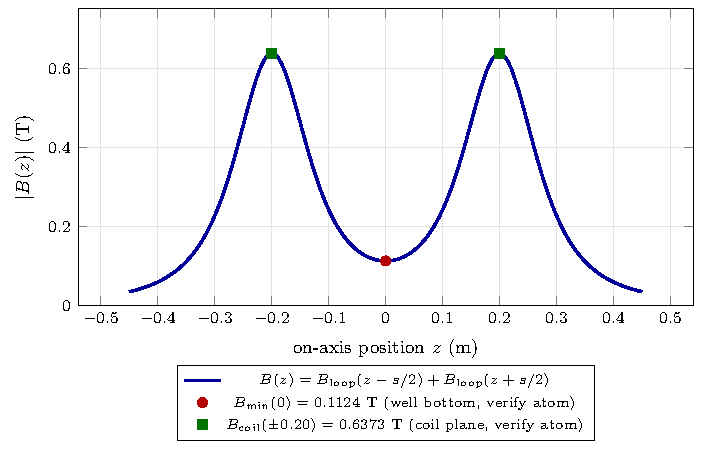
\includegraphics[width=0.82\linewidth]{figures/fig04_ioffe_profile.pdf}
\caption{On-axis $|B(z)|$ of the reference Ioffe--Pritchard mirror pair
($a=0.10$\,m, $I=10^5$\,A, $s=0.40$\,m, coils at $z=\pm0.20$\,m), from the
inherited Wheeler closed form (Eq.~\eqref{eq:conf-loop}) superposed via
Eq.~\eqref{eq:conf-mirror}. Because $s/a=4>1$, the centre $z=0$ is a true
on-axis \emph{minimum} (a magnetic bottle). The marked points are the
registered \tierGreen\ verify atoms: the well bottom
$B_{\min}(0)=0.1124$\,T (red) and the coil-plane maxima
$B_{\mathrm{coil}}(\pm0.20)=0.6373$\,T (green); their difference
$\Delta B=0.5249$\,T sets the $0.3526$\,K trap depth (PR~\#168).}
\label{fig:conf-app}
\end{figure}

% -------------------------------------------------------------------------
\subsection{Trap depth and the $\mu_B/k_B$ constant}
\label{app:conf-depth}

A low-field-seeker climbing from the well bottom $B_{\min}$ to the barrier
$B_{\mathrm{coil}}$ gains potential energy $\mu_B\,\Delta B$ with
$\Delta B=B_{\mathrm{coil}}-B_{\min}$. Expressed as an equivalent
temperature, the trap depth is
\begin{equation}
\frac{U_{\mathrm{depth}}}{k_B} \;=\; \frac{\mu_B}{k_B}\,\Delta B,
\qquad
\frac{\mu_B}{k_B} = 0.671714\ \mathrm{K/T},
\label{eq:conf-depth}
\end{equation}
the load-bearing constant of the stage (\verb|mu_b_over_kb|, the Bohr
magneton over Boltzmann's constant, CODATA-2018 \citep{mohr2018codata}). So a
$1$\,T well is $0.672$\,K deep, and the ALPHA-class $\sim$0.5\,T well is
$\sim$0.5\,K --- exactly the mK--K regime in which trapped antihydrogen lives
\citep{amole2014alphatrap}. For the reference pair the funnel computes
$B_{\min}=0.1124$\,T, $B_{\mathrm{coil}}=0.6373$\,T,
$\Delta B=0.5249$\,T, and trap depth $0.3526$\,K, all \tierGreen\
(Table~\ref{tab:conf-verify}).

\begin{table}[h]
\centering
\small
\setlength{\tabcolsep}{4pt}
\begin{tabular}{@{}l l r r r l@{}}
\toprule
\textbf{atom} & \textbf{args} & \textbf{expected} & \textbf{observed} & $|\Delta|$ & \textbf{tier} \\
\midrule
\verb|ioffe_loop_bz|       & (0.1,1e5,0.0) & $0.628319$ & $0.628319$ & $0$                  & \tierGreen \\
\verb|ioffe_mirror_bmin|   & (0.1,1e5,0.4) & $0.112397$ & $0.112397$ & $0$                  & \tierGreen \\
\verb|ioffe_mirror_bcoil|  & (0.1,1e5,0.4) & $0.637283$ & $0.637283$ & $0$                  & \tierGreen \\
\verb|ioffe_mirror_deltab| & (0.1,1e5,0.4) & $0.524886$ & $0.524886$ & $1.1\times10^{-16}$  & \tierGreen \\
\verb|ioffe_trap_depth_k|  & (0.524886)    & $0.352573$ & $0.352573$ & $1.7\times10^{-16}$  & \tierGreen \\
\verb|ioffe_trap_depth_k|  & (1.0)         & $0.671714$ & $0.671714$ & $2.2\times10^{-16}$  & \tierGreen \\
\verb|mu_b_over_kb|        & ()            & $0.671714$ & $0.671714$ & $2.2\times10^{-16}$  & \tierGreen \\
\bottomrule
\end{tabular}
\caption{Process \textcircled{\scriptsize 6} confinement atoms
(\texttt{companion/verify-ledger.json}, PR~\#168). The first three are the
single-loop on-axis field and the two-coil well bottom / barrier
(Eqs.~\eqref{eq:conf-loop}--\eqref{eq:conf-mirror}); the next two are the
trap depth for the reference $\Delta B$ and a $1$\,T reference well; the last
is the bare $\mu_B/k_B$ constant of Eq.~\eqref{eq:conf-depth}. The
$\sim10^{-16}$ residuals are single \texttt{pow}/division round-offs, not
modelling error.}
\label{tab:conf-verify}
\end{table}

\begin{lstlisting}
verify --expr ioffe_mirror_bmin(0.1,100000.0,0.4)=0.112397
  calc   = 0.112397 ~ expected 0.112397 (|Delta|=0.0 <= eps=1e-9)
  tier   = SUPPORTED-NUMERICAL (hexa-native libm-class recompute)
verify --expr ioffe_trap_depth_k(0.524886)=0.352573
  calc   = 0.352573 ~ expected 0.352573 (|Delta|=1.67e-16 <= eps=1e-9)
  tier   = SUPPORTED-NUMERICAL (hexa-native libm-class recompute)
verify --expr ioffe_mirror_deltab(0.1,100000.0,0.4)=0.9   # negative control
  calc   = 0.524886 != expected 0.9 (|Delta|=0.375114 > eps=1e-9)
  tier   = FALSIFIED (controlled negative)
\end{lstlisting}

% -------------------------------------------------------------------------
\subsection{The deferred GetDP FEM cross-check}
\label{app:conf-fem}

The closed-form Ioffe--Pritchard verify is fully landed (PR~\#168). The
inherited RTSC toolchain (Appendix~\ref{app:rtsc}) also carries a GetDP\,4.0
axisymmetric A--$\phi$ deck that could re-solve the same mirror geometry as a
finite-element field map and cross-check $B_{\min}$/$B_{\mathrm{coil}}$ against
the closed form, exactly as the RTSC solenoid was cross-checked (the M318
Wheeler-vs-FEM anchor). We deliberately keep that FEM re-solve out of scope
here to keep the verify tight: the on-axis quantities the trap depth depends
on are exactly the ones the Wheeler closed form gives in closed form, so the
FEM adds no closed-form precision at $r=0$. The deck and the runbook are
documented in Appendix~\ref{app:rtsc} for any reader who wishes to run it.

% -------------------------------------------------------------------------
\subsection{Honest scope}
\label{app:conf-scope}

This appendix closes the \emph{on-axis} field profile and the resulting trap
depth, not the full three-dimensional trap. The radial confinement of a true
Ioffe--Pritchard trap adds octupole (or higher) bars to close the field off
axis; their contribution to the depth at the reference geometry is not modelled
here. The numerical anchors ($a=0.10$\,m, $I=10^5$\,A) are representative, not
a sourced ALPHA apparatus geometry, and the depth is computed with the
ideal $\mu=\mu_B$ moment.
